\documentclass[a4paper,12pt]{article}
\usepackage[T1]{fontenc}
\usepackage[utf8]{inputenc}
\usepackage[czech,provide=*]{babel}
\usepackage{lmodern,amsmath,amssymb,graphicx,booktabs,array}
\usepackage[margin=25mm]{geometry}
\usepackage{pdfpages}
\usepackage{caption}

\usepackage[hidelinks]{hyperref}
\renewcommand{\arraystretch}{1.15}

% -----------------------------------------------------------------------------

\newcommand{\Autor}{Tomáš Levý}
\newcommand{\OsobniCislo}{A26B0314P}
\newcommand{\AkademickyRok}{ZS 2026/2027}
\newcommand{\Datum}{\today}
\newcommand{\CisloUlohy}{7}
\newcommand{\dd}{\mathrm{d}}

% -----------------------------------------------------------------------------

\begin{document}

\begin{titlepage}
\centering
\vspace*{10mm}
{\bfseries \Large Západočeská univerzita v Plzni\\[2mm] 
Fakulta aplikovaných věd\\[2mm] 
Katedra mechaniky\par}
\vspace{10mm}

\includegraphics[width=0.5\textwidth]{fig/ZCU_cmyk.pdf}

\vspace{25mm}
{\LARGE \color{gray!70!white}{\texttt{V Z O R O V Á}}}\\[5mm]
{\bfseries \LARGE Semestrální práce\\[30mm]
KME/KIN\par}
\vspace{5mm}
{\large Úloha č.\ \CisloUlohy\par}
\vfill
{
  \large
  \OsobniCislo
  \hfill
  \AkademickyRok
  \hfill
  \Autor
}
\vspace*{2mm}
\end{titlepage}


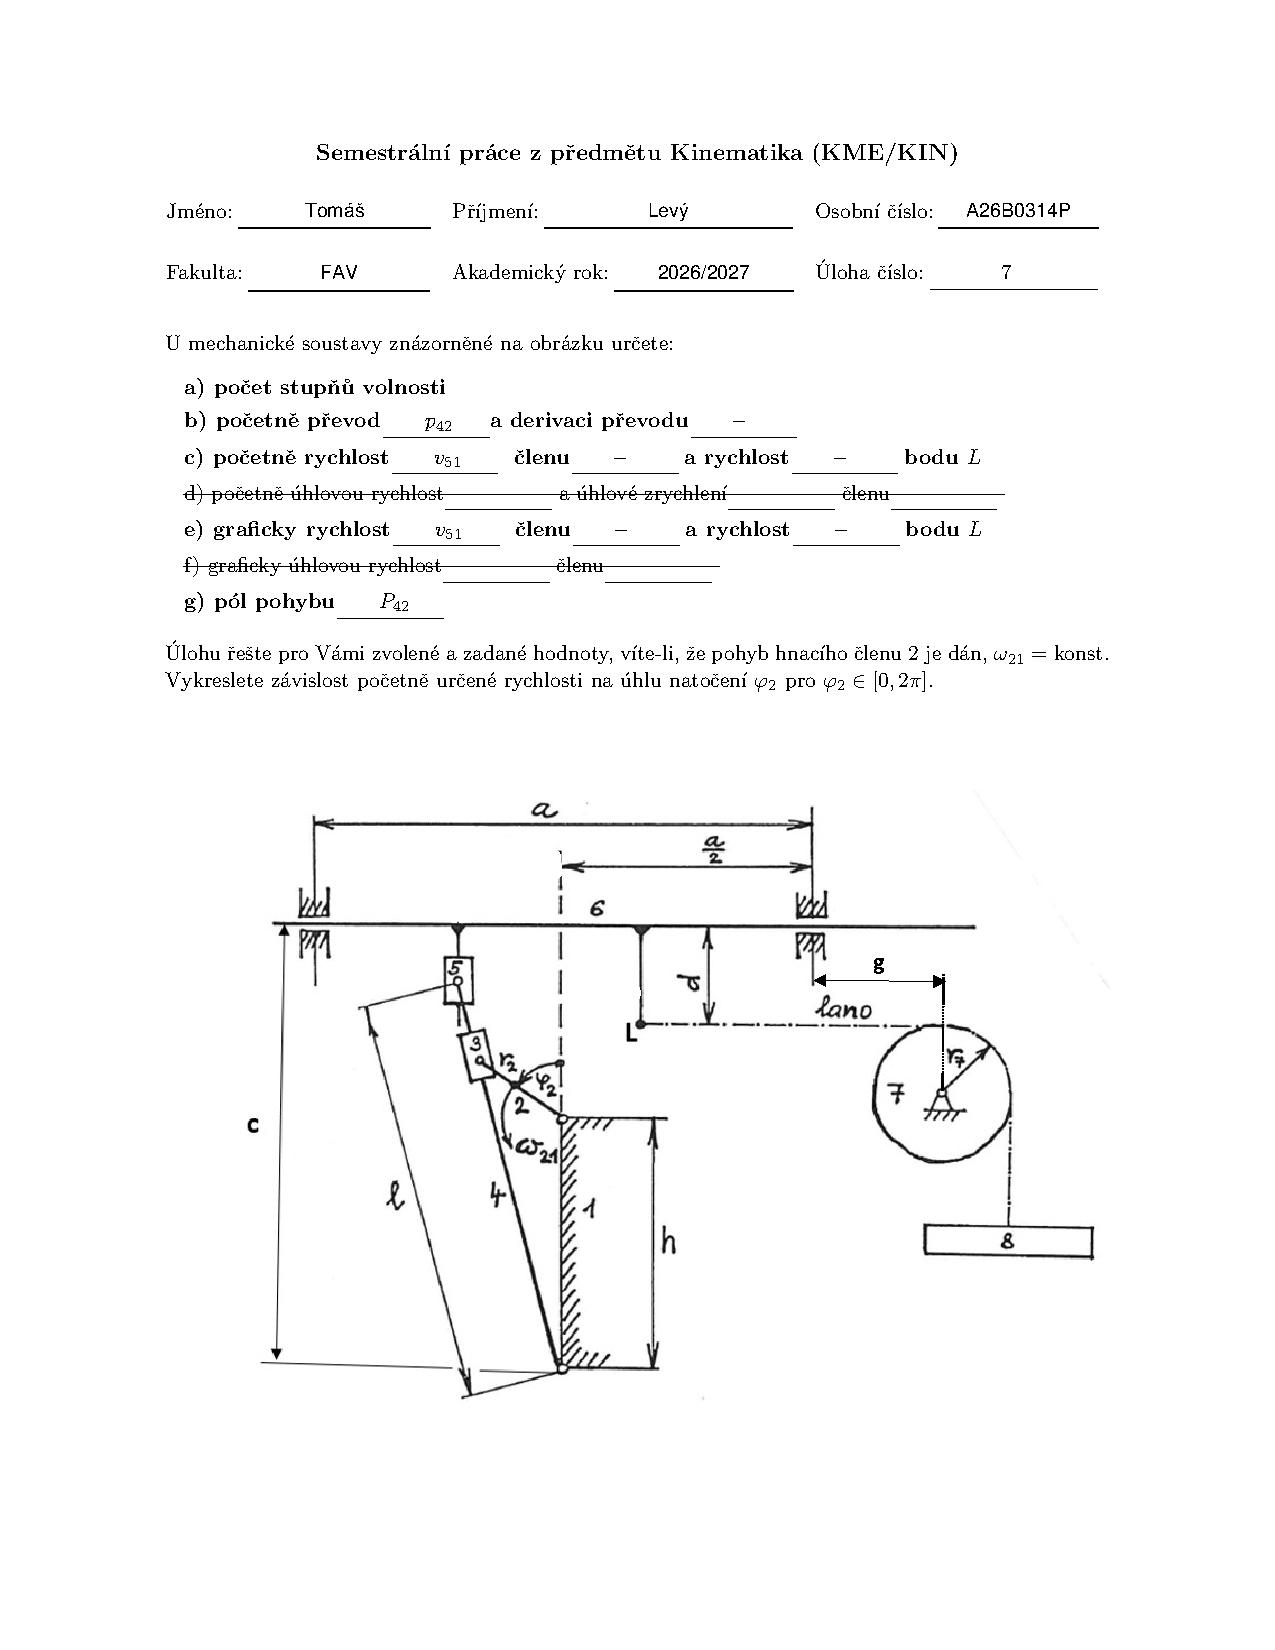
\includepdf[pages=1]{zadani.pdf}

\setcounter{page}{1}

% -----------------------------------------------------------------------------
\section{Počet stupňů volnosti}

Pro nalezení počtu stupňů volnosti zadaného mechanismu tvořeného členy 1 až 6 použijeme obecný vztah
\begin{equation}
  n=3(m-1)-2(r + p + v) - 1o,
\end{equation}
kde $m$ je celkový počet členů soustavy a symboly $r, p, v, o$ označují počet rotačních, posuvných, valivých a obecných kinematických dvojic (KD). Člen 1 je zde rám a $m=6$. Odpovídající vazby jsou:
\begin{center}
  \begin{tabular}{cc}\toprule
    Členy & Typ KD\\\midrule
    1--2 & rotační\\
    2--3 & rotační\\
    1--4 & rotační\\
    3--4 & posuvná\\
    4--5 & rotační\\
    5--6 & posuvná\\
    6--1 & posuvná\\\bottomrule
  \end{tabular}
\end{center}
tj. čtyři rotační a tři posuvné KD, proto
\begin{equation}
  \boxed{
    n=3(6-1)-2(4+3)=1.
  }
\end{equation}

Při napnutém a nepružném laně a bez prokluzu lana na kladce jsou posuv závaží 8 a natočení kladky 7 jednoznačně určeny posuvem členu 6. Tyto členy proto nepřidávají další nezávislý stupeň volnosti.

\newpage
% -----------------------------------------------------------------------------
\section{Určení převodu \texorpdfstring{$p_{42}$}{p42}}

Předpokládejme zadané rozměry $r_2$, $\ell$ a $h$. Pro dané $\omega_{21} = \mathrm{konst}$ koná klika 2 rovnoměrný rotační pohyb, a tedy $\alpha_{21} = 0$ a $\varphi_{2} = \varphi_{2,0}+\omega_{21}t$. 
Označme $\varphi_4$ úhel natočení vahadla 4 vůči rámu 1.
Pomocí trigonometrické metody, viz obr. \ref{f:pocetne}, získáváme z geometrie mechanismu
\begin{equation}
  \mathrm{tg}\varphi_4=\frac{r_2\sin\varphi_2}{h+r_2\cos\varphi_2}.
\end{equation}
Pro $h>r_2$ je jmenovatel vždy kladný a lze tedy psát
\begin{equation}
 \varphi_4 = \mathrm{arctg}\frac{r_2\sin\varphi_2}{h+r_2\cos\varphi_2},
\end{equation}
což je současně zdvihová funkce $\varphi_4 = f_{42}(\varphi_2)$.
Pro převod v případě rotujících členů soustavy obecně platí
\begin{equation}
  p_{ik} = \frac{\dd f_{ik}(\varphi_k)}{\dd \varphi_k},
\end{equation}
a tedy
\begin{align}
  p_{42}&= \frac{\dd\varphi_4}{\dd\varphi_2}
         = \frac{1}{1 + \left( \dfrac{r_2 \sin\varphi_2}{h + r_2 \cos\varphi_2} \right)^2}
           \frac
           {r_2 \cos\varphi_2 \left(h + r_2\cos\varphi_2 \right) + r_2^2 \sin^2\varphi_2}
           {\left( h + r_2 \cos\varphi_2 \right)^2}\\
        &=
  \boxed{
           \frac{r_2(r_2+h\cos\varphi_2)}{h^2 + 2 h r_2 \cos\varphi_2 + r_2^2}.
  }
\end{align}

\begin{figure}[!h]
  \centering
  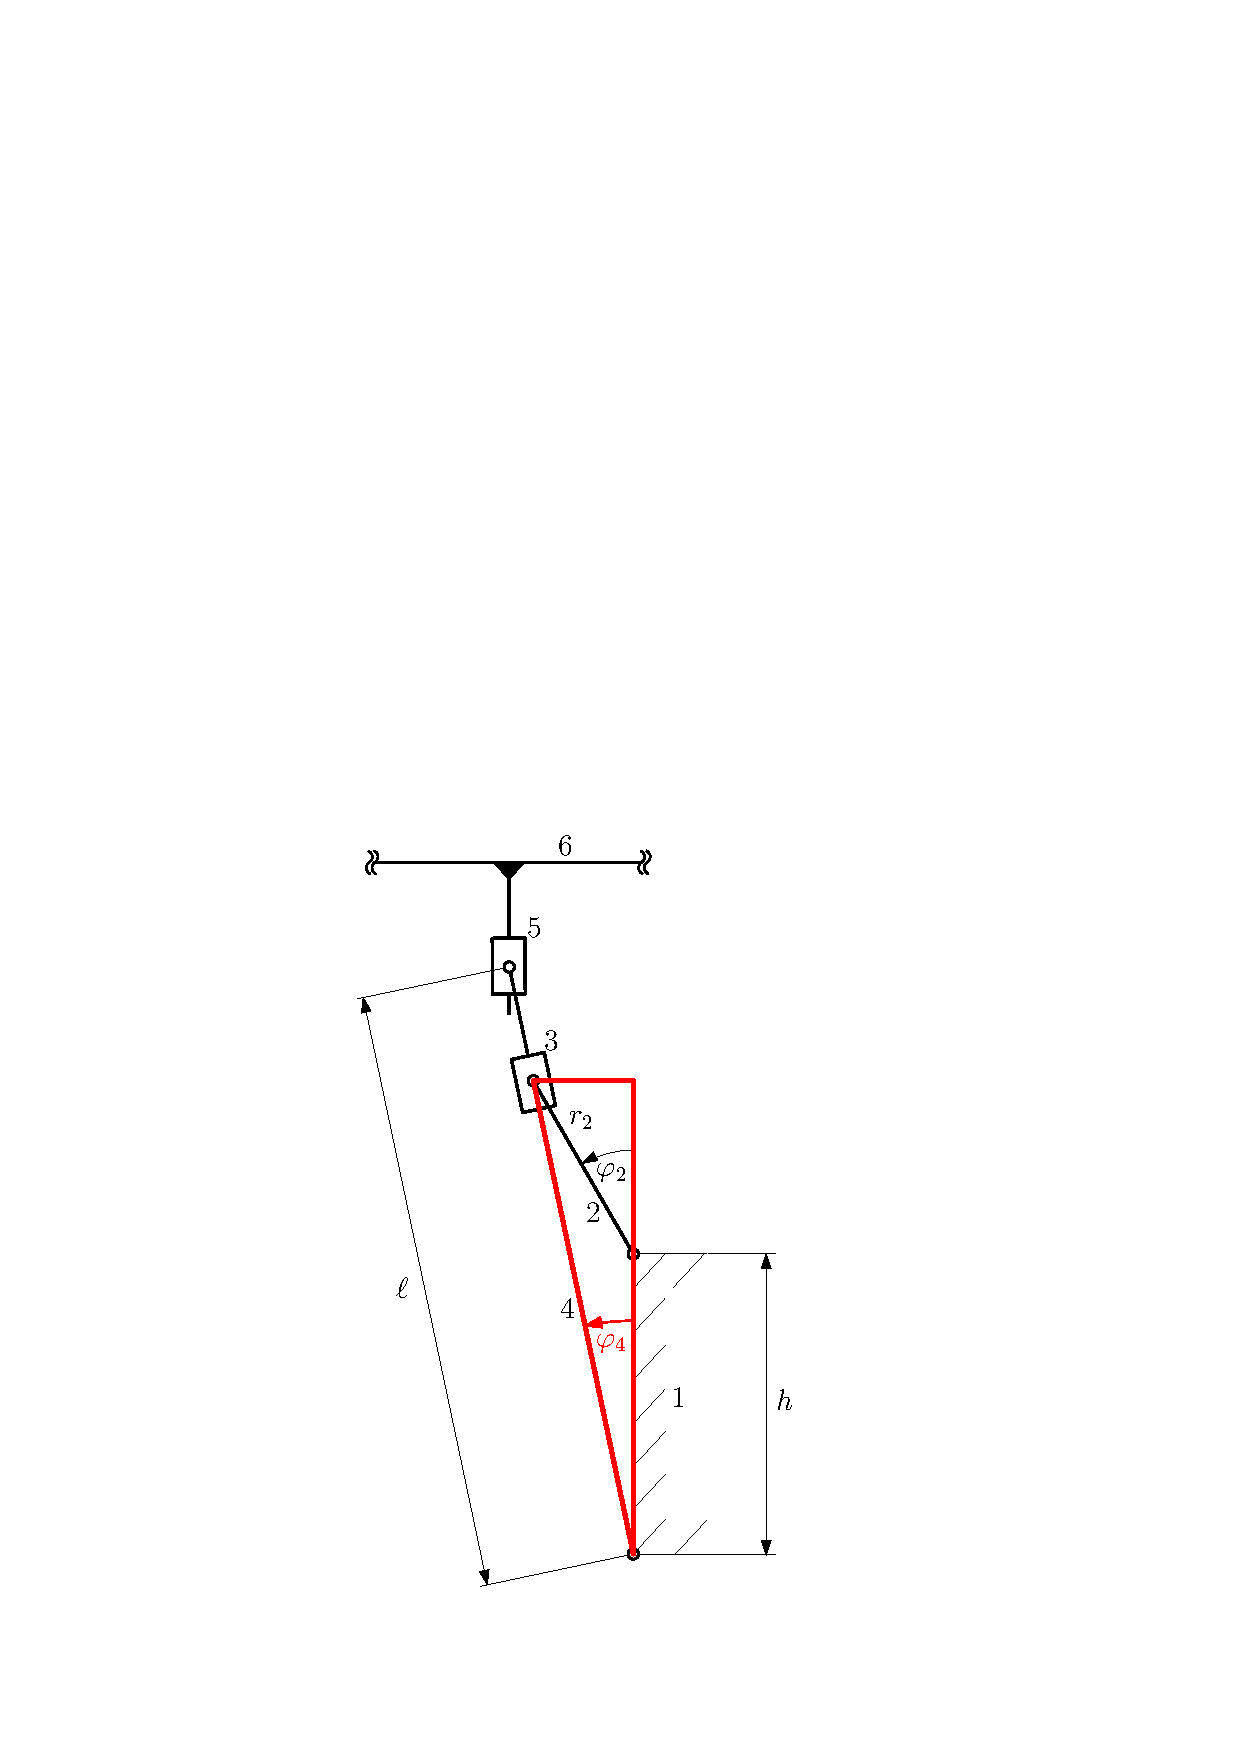
\includegraphics[width=0.35\textwidth]{fig/pocetne.pdf}
  \caption{Úhel $\varphi_4$ a naznačení trigonometrické metody}
  \label{f:pocetne}
\end{figure}


\newpage
% -----------------------------------------------------------------------------
\section{Analytické určení rychlosti \texorpdfstring{$v_{51}$}{v51}}
Člen 5 koná vůči rámu posuvný pohyb, a proto mají všechny jeho body stejný vektor rychlosti. V rotační KD 4--5 mají oba členy ve společném bodě stejnou rychlost. 
Vzhledem k rotačnímu pohybu členu 4 potom platí
\begin{equation}
  v_{51} = \ell \omega_{41}.
\end{equation}
Ze znalosti převodu $p_{42}$ dále získáváme
\begin{equation}
  \omega_{41} = \frac{\dd \varphi_4}{\dd t}
              = \frac{\dd \varphi_4}{\dd \varphi_2} \frac{\dd \varphi_2}{\dd t}
              = p_{42} \omega_{21},
\end{equation}
a tedy
\begin{equation}
  \boxed{
    v_{51} = \frac{\ell r_2(r_2+h\cos\varphi_2)}{h^2 + 2 h r_2 \cos\varphi_2 + r_2^2} \omega_{21}.
  }
  \label{eq:v51}
\end{equation}
Pro zvolené hodnoty
\begin{itemize}
  \item $h = 9 \, \mathrm{m}$,
  \item $r_2 = 6 \, \mathrm{m}$,
  \item $\ell = 18 \, \mathrm{m}$,
  \item $\varphi_2 = 30^\circ$,
  \item $\omega_{21} = 1{,}2\, \mathrm{rad}\cdot\mathrm{s}^{-1}$,
\end{itemize}
tak po dosazení do vztahu \eqref{eq:v51} dostáváme
\begin{equation}
  \boxed{
    v_{51} = 8{,}492 \, \mathrm{m}\cdot\mathrm{s}^{-1}.
  }
  \label{eq:v51eval}
\end{equation}
Závislost hledané rychlosti $v_{51}$ na úhlu natočení $\varphi_2$ kliky $2$ daná vztahem \eqref{eq:v51} je vynesena na obr. \ref{f:graf}.
Znaménko rychlosti $v_{51}$ vyjadřuje smysl pohybu: kladné hodnoty odpovídají rostoucímu úhlu $\varphi_4$, záporné jeho poklesu. Nulové hodnoty odpovídají okamžikům obrácení pohybu vahadla.
Detail v okolí zvoleného úhlu natočení $\varphi_2 = 30^\circ$ poté odpovídá vyčíslené hodnotě \eqref{eq:v51eval}.

\begin{figure}[!h]
  \centering
  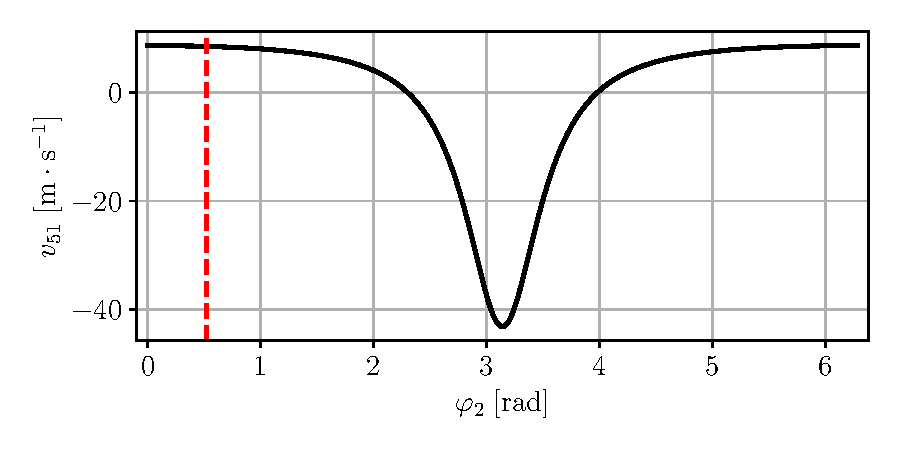
\includegraphics[width=0.66\textwidth]{script/v51.pdf}
  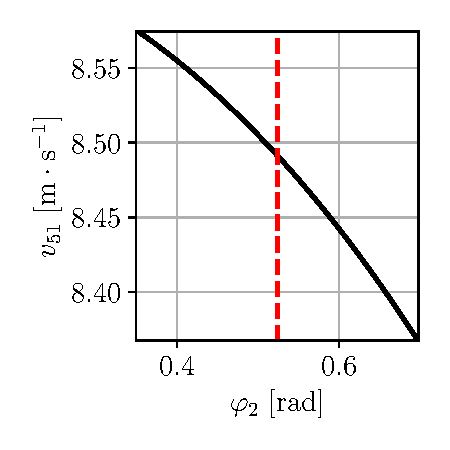
\includegraphics[width=0.33\textwidth]{script/v51_detail.pdf}
  \caption{Graf závislosti $v_{51}(\varphi_2)$ pro $\varphi_2 \in \left[ 0, 2\pi \right]$ vlevo a detail v okolí $\varphi_2 = 30^\circ$ vpravo}
  \label{f:graf}
\end{figure}


\newpage
% -----------------------------------------------------------------------------
\section{Grafické určení rychlosti \texorpdfstring{$v_{51}$}{v51}}

Pro grafickou konstrukci na obr.~\ref{f:graficky} volíme měřítko délek tak, že jeden dílek čtvercové sítě odpovídá délce $1\,\mathrm{m}$, a měřítko rychlostí tak, že jeden dílek odpovídá rychlosti $1\,\mathrm{m\,s^{-1}}$. Při uvážení výše uvedených hodnot nalezneme rychlost $v_{51}$ graficky následujícím postupem.

\begin{figure}[!h]
  \centering
  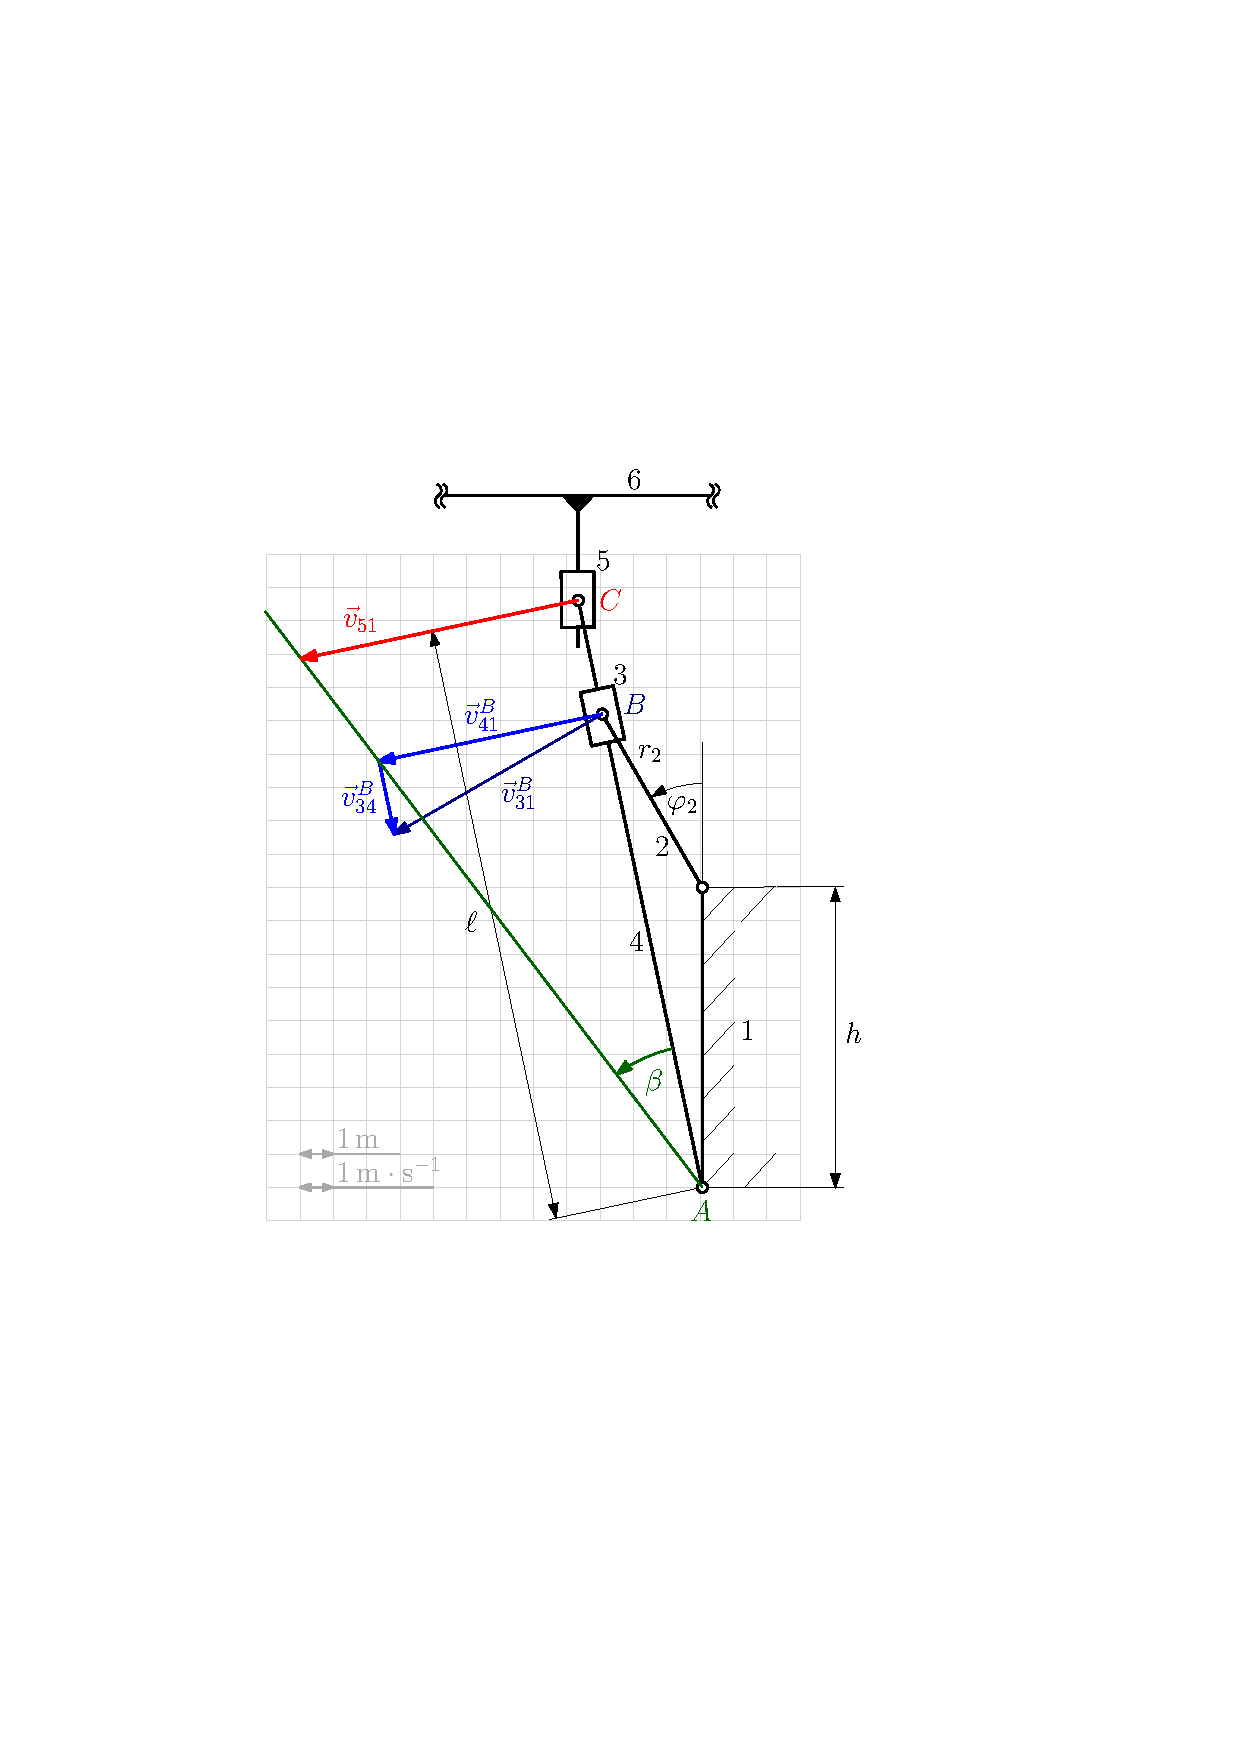
\includegraphics[width=0.5\textwidth]{fig/graficky.pdf}
  \caption{Grafické řešení rychlosti $v_{51}$}
  \label{f:graficky}
\end{figure}

\begin{enumerate}
  \item Nejprve sestrojíme rychlost kliky 2 v místě polohy objímky 3, tj. v bodě $B$. Vzhledem k rotačnímu charakteru pohybu má směr kolmý na kliku 2 a velikost odpovídá
  \begin{equation}
    v_{31}^B = r_2 \omega_{21} = 6 \cdot 1{,}2 = 7{,}2\, \mathrm{m}\cdot \mathrm{s}^{-1}.
  \end{equation}
  \item S uvážením rozkladu pohybu $31 = 34 + 41$ pak pro vektor rychlosti $\vec{v}_{31}^B$ rovněž platí
  \begin{equation}
    \vec{v}_{31}^B = \vec{v}_{34}^B + \vec{v}_{41}^B,
  \end{equation}
  kde $\vec{v}_{34}^B$ je vektor rychlosti posuvného pohybu členu 3 po členu 4 v místě $B$ a $\vec{v}_{41}^B$ je vektor rychlosti rotačního pohybu vahadla 4 vůči rámu 1 v místě $B$. Charakter obou pohybů plně určuje směr těchto vektorů:
  \begin{align}
    \vec{v}_{34}^B \,||\, {AB}, \qquad
    \vec{v}_{41}^B \perp {AB}.
  \end{align}
  \item Konečně, vektor rychlosti $\vec{v}_{51} \equiv \vec{v}_{51}^C$ je poté viděn z bodu $A$ pod stejným úhlem $\beta$ jako vektor $\vec{v}_{41}^B$ a platí
  \begin{align}
    \vec{v}_{41}^B \,||\, \vec{v}_{51}.
  \end{align}
\end{enumerate}
Po odměření získáváme
\begin{equation}
  \boxed{
    v_{51} \approx 8{,}5 \, \mathrm{m}\cdot\mathrm{s}^{-1},
  }
\end{equation}
což je v souladu s početním výsledkem daným rovnicí \eqref{eq:v51eval}.


\newpage
% -----------------------------------------------------------------------------
\section{Nalezení pólu relativního pohybu \texorpdfstring{$P_{42}$}{P42}}
Pro nalezení pólu relativního pohybu $P_{42}$ použijeme rozklady pohybu
\begin{align*}
  {\color{red}{42 = 43 + 32}} \qquad \mathrm{a} \qquad {\color{blue}{42 = 41 + 12}}.
\end{align*}

\begin{itemize}
  \item Relativní pohyb $32$ je rotační se středem rotace na objímce 3, čímž je současně dána poloha pólu $P_{32}$.
  \item Pohyb $43$ vahadla 4 vůči objímce 3~je posuvný. Pólem pohybu je tedy úběžný bod ležící na kolmici ke směru pohybu.
  \item Spojením těchto dvou pólů získáváme přímku $n_{P_{42}}$, na které pól $P_{42}$ musí ležet.
  \item Pohyby $41$ a $12$ jsou oba rotační a $P_{41}$ tedy leží v pevném kloubu vahadla 4 a $P_{12}$ v pevném kloubu kliky 2. Na spojnici pólů $P_{41}$ a $P_{12}$ musí rovněž ležet hledaný pól $P_{42}$. Tím je jeho poloha jednoznačně určena.
\end{itemize}

\begin{figure}[!h]
    \centering
    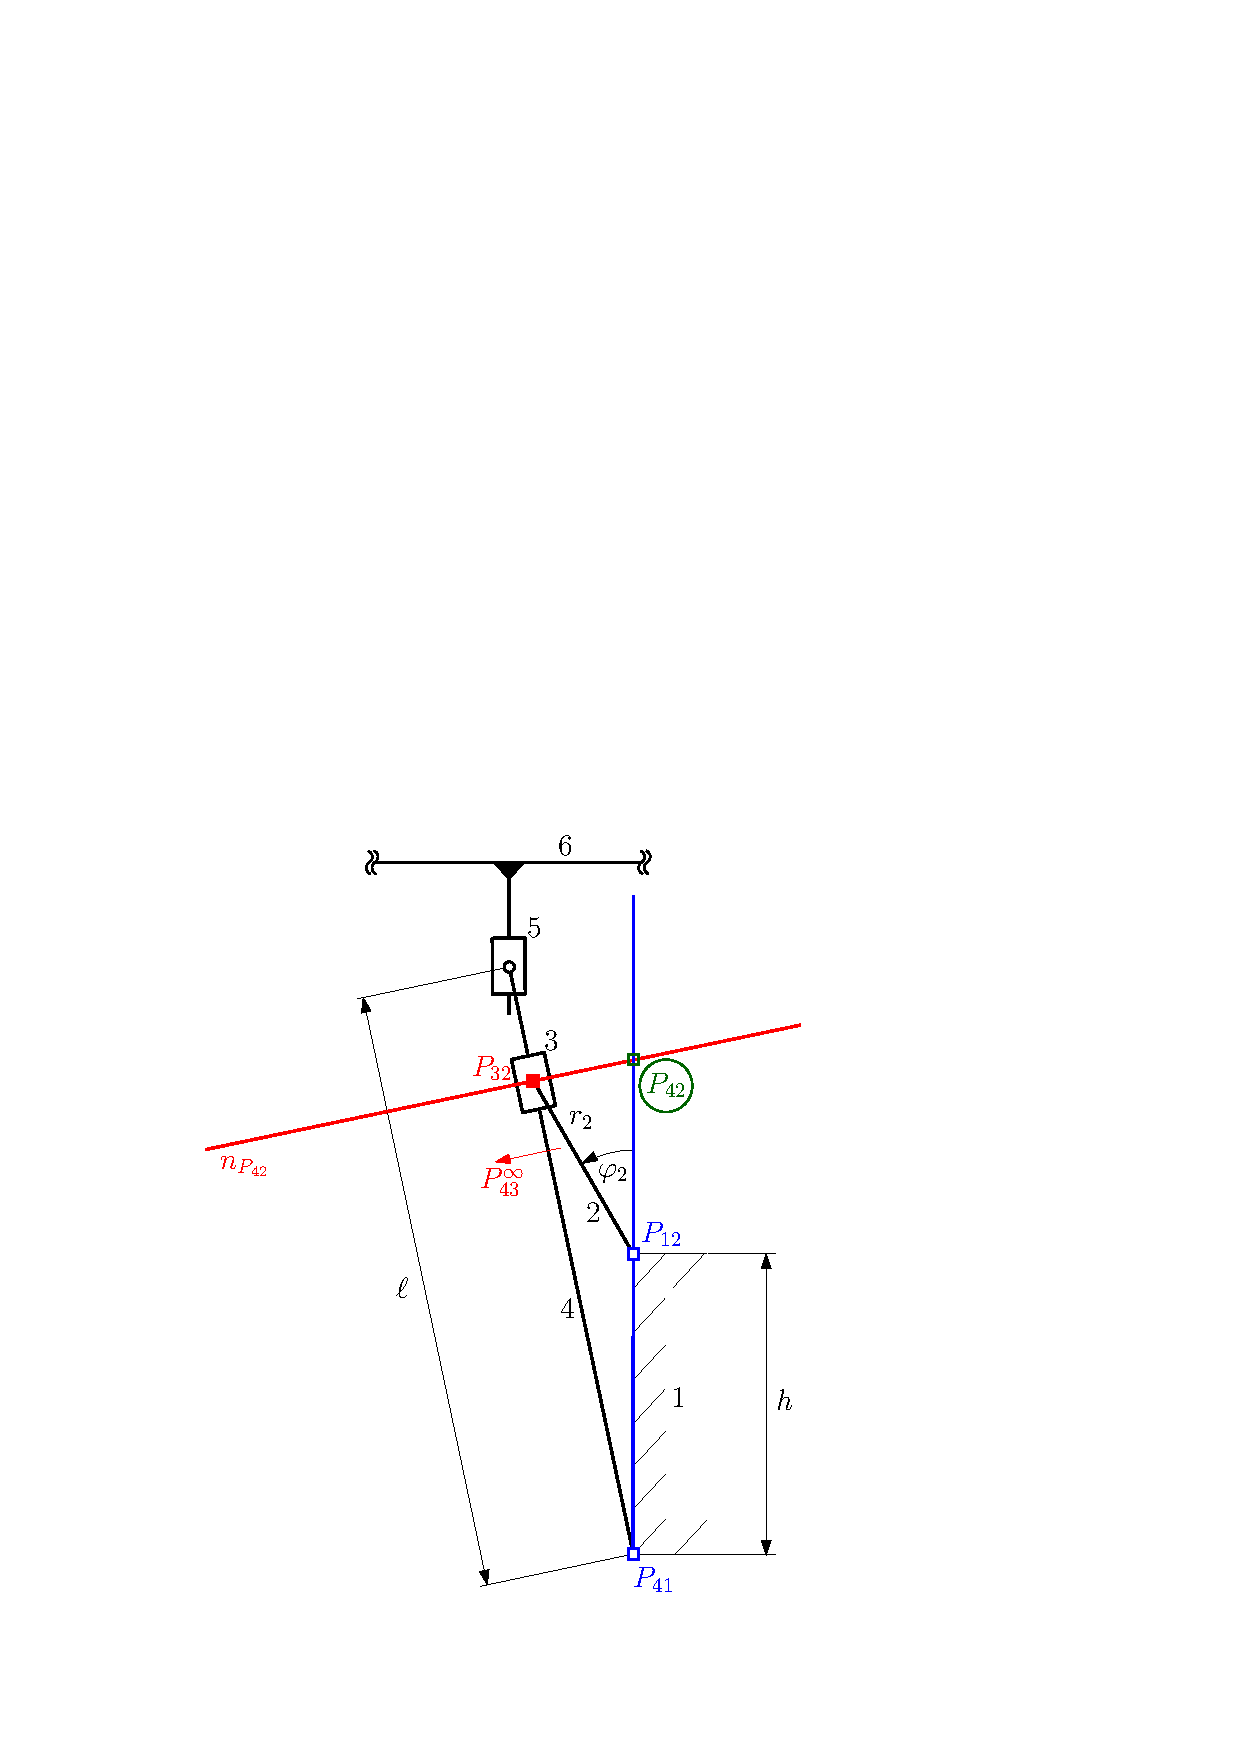
\includegraphics[width=0.5\textwidth]{fig/pol.pdf}
    \caption{Nalezení pólu pohybu $P_{42}$}
    \label{f:pol}
  \end{figure}

\end{document}
